\documentclass[aspectratio=169,10pt]{beamer}

\usepackage[T1]{fontenc}
\usepackage[utf8]{inputenc}
\usepackage{lmodern}
\usepackage{microtype}
\usepackage{booktabs}
\usepackage{array}
\usepackage{colortbl}
\usepackage{xcolor}
\usepackage{tikz}
\usepackage{amsmath}
\usepackage{amssymb}
\usepackage{tabularx}
\usepackage{multirow}
\usepackage{ragged2e}
\usepackage{calc}

\usetikzlibrary{arrows.meta,shapes.geometric,positioning,fit,backgrounds,calc}

%% ── Palette ──────────────────────────────────────────────────
\definecolor{Navy}{RGB}{15,32,67}
\definecolor{Teal}{RGB}{0,158,143}
\definecolor{TealLight}{RGB}{220,245,243}
\definecolor{Amber}{RGB}{230,140,0}
\definecolor{Snow}{RGB}{250,251,253}
\definecolor{Steel}{RGB}{95,110,135}
\definecolor{Crimson}{RGB}{196,48,43}

%% ── Beamer Theme ─────────────────────────────────────────────
\usetheme{default}
\setbeamertemplate{navigation symbols}{}

\setbeamercolor{normal text}{fg=Navy,bg=Snow}
\setbeamercolor{structure}{fg=Teal}
\setbeamercolor{frametitle}{fg=white,bg=Navy}
\setbeamercolor{block title}{fg=white,bg=Navy}
\setbeamercolor{block body}{fg=Navy,bg=TealLight}
\setbeamercolor{block title alerted}{fg=white,bg=Crimson}
\setbeamercolor{block body alerted}{fg=Navy,bg=Crimson!10}
\setbeamercolor{block title example}{fg=white,bg=Teal}
\setbeamercolor{block body example}{fg=Navy,bg=TealLight}
\setbeamercolor{itemize item}{fg=Teal}
\setbeamercolor{enumerate item}{fg=Teal}

\setbeamerfont{frametitle}{size=\large,series=\bfseries}
\setbeamerfont{block title}{size=\small,series=\bfseries}

\setbeamertemplate{itemize item}{\color{Teal}\small$\blacktriangleright$}
\setbeamertemplate{itemize subitem}{\color{Teal}\footnotesize$\triangleright$}

\setbeamertemplate{frametitle}{%
  \nointerlineskip
  \begin{beamercolorbox}[wd=\paperwidth,ht=0.58cm,dp=0.12cm,
      leftskip=0.5cm,rightskip=0.4cm]{frametitle}%
    \usebeamerfont{frametitle}\insertframetitle
    \ifx\insertframesubtitle\empty\else
      \hfill{\color{TealLight}\small\itshape\insertframesubtitle}%
    \fi
  \end{beamercolorbox}%
  {\color{Teal}\rule{\paperwidth}{1.5pt}}%
}

\setbeamertemplate{footline}{%
  \begin{beamercolorbox}[wd=\paperwidth,ht=0.38cm,dp=0.12cm,
      leftskip=0.5cm,rightskip=0.5cm]{structure}%
    {\color{Steel}\tiny OF-RHM Moving Target Defense \textbullet\ First Review}%
    \hfill
    {\color{Steel}\tiny\insertframenumber\,/\,\inserttotalframenumber}%
  \end{beamercolorbox}%
}

%% ── Background helpers ───────────────────────────────────────
\newcommand{\lightbg}{%
  \setbeamertemplate{background}{%
    
\begin{tikzpicture}
      \useasboundingbox(0,0) rectangle(\paperwidth,\paperheight);
      \fill[Snow] (0,0) rectangle(\paperwidth,\paperheight);
      \fill[Teal!10] (0,0) rectangle(\paperwidth,0.5cm);
      \fill[Navy!4] (\paperwidth-1.2cm,\paperheight) --
        (\paperwidth,\paperheight) --
        (\paperwidth,\paperheight-1.2cm) -- cycle;
    \end{tikzpicture}%
  }%
}

\newcommand{\darkbg}{%
  \setbeamertemplate{background}{%
    
\begin{tikzpicture}
      \useasboundingbox(0,0) rectangle(\paperwidth,\paperheight);
      \fill[Navy] (0,0) rectangle(\paperwidth,\paperheight);
      \fill[Teal!70!black] (0,0) rectangle(\paperwidth,0.7cm);
      \fill[Teal!70!black,opacity=0.25]
        (0,\paperheight-0.7cm) rectangle(\paperwidth,\paperheight);
      \fill[Teal!20,opacity=0.06]
        (\paperwidth*0.78,\paperheight*0.5) circle(3cm);
    \end{tikzpicture}%
  }%
}

\lightbg

%% ═════════════════════════════════════════════════════════════
\begin{document}
%% ═════════════════════════════════════════════════════════════

%% ── TITLE ────────────────────────────────────────────────────
{\darkbg
\setbeamertemplate{footline}{}
\begin{frame}[plain]
  \vspace{0.55cm}
  \begin{columns}[T]
    \begin{column}{0.62\textwidth}
      {\color{Teal}\footnotesize\bfseries
        COMPUTER NETWORKS \textbullet\ FIRST REVIEW PRESENTATION}
      \vspace{0.3cm}\\
      {\color{white}\LARGE\bfseries
        Moving Target Defense\\[5pt]
        Using OpenFlow Random\\[5pt]
        Host Mutation (OF-RHM)}
      \vspace{0.35cm}\\
      {\color{TealLight}\small\itshape
        Proactive Security via Continuous IP Randomisation}
      \vspace{0.65cm}\\
      {\color{white}\small\bfseries Presented by:}\\[3pt]
      {\color{TealLight}\small Aditi Sriram}
      \vspace{0.3cm}\\
      {\color{white}\small\bfseries Date:\
        \color{TealLight}August 2026 \quad}
      {\color{white}\small\bfseries Course:\
        \color{TealLight}Computer Networks}
    \end{column}
    \begin{column}{0.35\textwidth}
      \vspace{0.4cm}\centering
      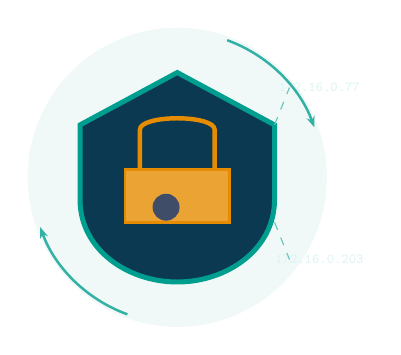
\begin{tikzpicture}[scale=0.95]
        % outer glow ring
        \fill[Teal!30,opacity=0.2] (1.6,1.6) circle(2.0cm);
        % shield body
        \fill[Navy!80!Teal]
          (1.6,3.0) -- (0.3,2.3) -- (0.3,1.3)
          to[out=270,in=180] (1.6,0.2)
          to[out=0,in=270] (2.9,1.3)
          -- (2.9,2.3) -- cycle;
        \draw[Teal,line width=1.8pt]
          (1.6,3.0) -- (0.3,2.3) -- (0.3,1.3)
          to[out=270,in=180] (1.6,0.2)
          to[out=0,in=270] (2.9,1.3)
          -- (2.9,2.3) -- cycle;
        % lock shackle
        \draw[Amber,line width=1.6pt,rounded corners=5pt]
          (1.1,1.6) -- (1.1,2.05)
          to[out=90,in=90] (2.1,2.05)
          -- (2.1,1.6);
        % lock body
        \fill[Amber!80] (0.9,1.0) rectangle (2.3,1.7);
        \draw[Amber,line width=1pt] (0.9,1.0) rectangle (2.3,1.7);
        \fill[Navy!80] (1.45,1.2) circle(0.18cm);
        % rotating VIP labels
        \node[color=TealLight,font=\tiny\bfseries] at (3.5,2.8)
          {\texttt{172.16.0.77}};
        \node[color=TealLight,font=\tiny\bfseries] at (3.5,0.5)
          {\texttt{172.16.0.203}};
        \draw[Teal!60,dashed,thin] (2.9,2.3) -- (3.1,2.8);
        \draw[Teal!60,dashed,thin] (2.9,1.0) -- (3.1,0.5);
        % rotation arrows
        \draw[-{Stealth[length=4pt]},Teal!80,line width=0.9pt]
          ($(1.6,1.6)+(70:1.95cm)$) arc(70:20:1.95cm);
        \draw[-{Stealth[length=4pt]},Teal!80,line width=0.9pt]
          ($(1.6,1.6)+(250:1.95cm)$) arc(250:200:1.95cm);
      \end{tikzpicture}
    \end{column}
  \end{columns}
\end{frame}}

%% ── OUTLINE ──────────────────────────────────────────────────
\begin{frame}{Outline}
  \vspace{0.3cm}
  \begin{columns}[T]
    \begin{column}{0.48\textwidth}
      \begin{itemize}\setlength\itemsep{7pt}\small
        \item[\color{Teal}\bfseries 01] Introduction
        \item[\color{Teal}\bfseries 02] Literature Review
        \item[\color{Teal}\bfseries 03] Objectives \& Significance
        \item[\color{Teal}\bfseries 04] Problem Statement
        \item[\color{Teal}\bfseries 05] Key Deliverables
        \item[\color{Teal}\bfseries 06] Methodology
      \end{itemize}
    \end{column}
    \begin{column}{0.48\textwidth}
      \begin{itemize}\setlength\itemsep{7pt}\small
        \item[\color{Teal}\bfseries 07] Progress So Far
        \item[\color{Teal}\bfseries 08] Challenges \& Risks
        \item[\color{Teal}\bfseries 09] Next Steps
        \item[\color{Teal}\bfseries 10] Conclusion
        \item[\color{Teal}\bfseries 11] Q\,\&\,A
        \item[\color{Teal}\bfseries 12] References
      \end{itemize}
    \end{column}
  \end{columns}
\end{frame}

%% ══════════════════════════════════════════════════════════════
%% 01 INTRODUCTION
%% ══════════════════════════════════════════════════════════════
\begin{frame}{Introduction}{Background \& Context}
  \begin{columns}[T]
    \begin{column}{0.55\textwidth}
      \begin{itemize}\setlength\itemsep{6pt}
        \item Every device on a network has a permanent \textbf{IP address} --- its unique identity, like a home address.
        \item In a normal network these addresses \textbf{never change}, giving attackers a stable target to study.
        \item An attacker runs a \textbf{scan} once, records all live IPs and open services, then comes back days later to attack --- the map is \emph{still valid}.
        \item Traditional defences (firewalls, intrusion detection) are \textbf{reactive} --- they act \emph{after} an attack has already begun.
        \item This project applies \textbf{Moving Target Defense (MTD)}: proactively change the network's visible surface so reconnaissance becomes useless.
      \end{itemize}
    \end{column}
    \begin{column}{0.41\textwidth}
      \vspace{0.2cm}
      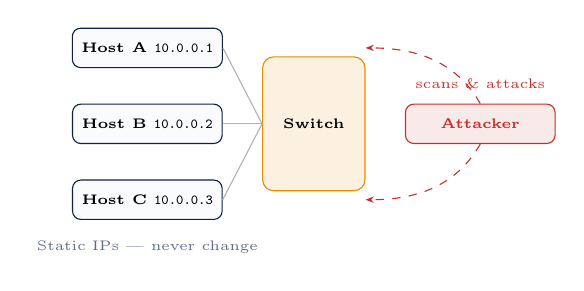
\begin{tikzpicture}[
          host/.style={draw=Navy,fill=Snow,rounded corners=3pt,
            minimum width=1.9cm,minimum height=0.5cm,
            font=\tiny\bfseries,align=center},
          sw/.style={draw=Amber,fill=Amber!12,rounded corners=4pt,
            minimum width=1.3cm,minimum height=1.7cm,
            font=\tiny\bfseries,align=center},
          atk/.style={draw=Crimson,fill=Crimson!10,rounded corners=3pt,
            minimum width=1.9cm,minimum height=0.5cm,
            font=\tiny\bfseries,text=Crimson,align=center}]
        \node[host](h1){Host A \texttt{10.0.0.1}};
        \node[host,below=0.45cm of h1](h2){Host B \texttt{10.0.0.2}};
        \node[host,below=0.45cm of h2](h3){Host C \texttt{10.0.0.3}};
        \node[sw,right=0.5cm of h2](sw){Switch};
        \node[atk,right=0.5cm of sw](atk){Attacker};
        \foreach \n in {h1,h2,h3}
          \draw[Navy!35] (\n.east) -- (sw.west);
        \draw[Crimson,dashed,-{Stealth[length=3pt]}]
          (atk.north) to[out=120,in=0] (sw.east |- h1.east);
        \draw[Crimson,dashed,-{Stealth[length=3pt]}]
          (atk.south) to[out=240,in=0] (sw.east |- h3.east);
        \node[font=\tiny,text=Crimson,above=2pt of atk]{scans \& attacks};
        \node[font=\tiny,text=Steel,below=4pt of h3]
          {Static IPs — never change};
      \end{tikzpicture}
    \end{column}
  \end{columns}
\end{frame}

\begin{frame}{Introduction}{The Problem with Static Addresses}
  \begin{columns}[T]
    \begin{column}{0.5\textwidth}
      \begin{block}{The Attacker's Advantage}
        \begin{itemize}\small\setlength\itemsep{5pt}
          \item Run a port scan once $\rightarrow$ complete map of all IPs and services.
          \item Return any time --- the map is \textbf{still accurate} because addresses never change.
          \item \textbf{Defender must be right every day.} Attacker only needs to succeed once.
        \end{itemize}
      \end{block}
      \vspace{0.25cm}
      \begin{alertblock}{By the Numbers}
        \small Scanning 254 addresses with \texttt{nmap} takes \textbf{under 5 seconds}. Without MTD, that intelligence remains valid \textbf{indefinitely}.
      \end{alertblock}
    \end{column}
    \begin{column}{0.46\textwidth}
      \vspace{0.15cm}
      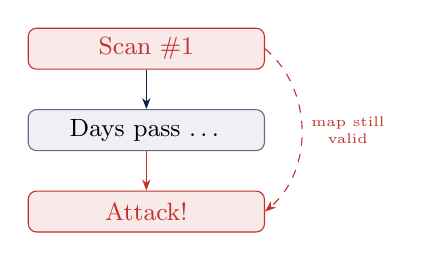
\begin{tikzpicture}[scale=0.88,
          ev/.style={draw,rounded corners=3pt,minimum width=3cm,
            minimum height=0.52cm,font=\small,align=center}]
        \node[ev,fill=Crimson!10,draw=Crimson,text=Crimson](s1){Scan \#1};
        \node[ev,fill=Steel!10,draw=Steel,below=0.5cm of s1](w){Days pass \ldots};
        \node[ev,fill=Crimson!10,draw=Crimson,text=Crimson,
              below=0.5cm of w](atk){Attack!};
        \draw[-{Stealth[length=4pt]},Navy] (s1)--(w);
        \draw[-{Stealth[length=4pt]},Crimson] (w)--(atk);
        \draw[Crimson,dashed,-{Stealth[length=4pt]},bend left=50]
          (s1.east) to node[right,font=\tiny,text=Crimson,align=center]
            {map still\\valid} (atk.east);
      \end{tikzpicture}
      \vspace{0.3cm}
      \begin{exampleblock}{Our Solution}
        \centering\small
        \textbf{Move the target} --- change all visible IPs every 30 seconds. Any map the attacker collects becomes instantly outdated.
      \end{exampleblock}
    \end{column}
  \end{columns}
\end{frame}

\begin{frame}{Introduction}{Moving Target Defense --- The Core Idea}
  \begin{columns}[T]
    \begin{column}{0.55\textwidth}
      \begin{itemize}\setlength\itemsep{6pt}
        \item Each host is given a \textbf{Virtual IP (VIP)} --- a fake address shown to the outside world; the real address stays hidden.
        \item Every \textbf{30 seconds}, all VIPs are replaced with new random ones from a pool.
        \item Legitimate traffic is \textbf{unaffected} --- the switch rewrites addresses transparently.
        \item An attacker who scans and records \texttt{172.16.0.77} will find a \emph{completely different} VIP next time --- their map is worthless.
        \item Scan detection triggers an \textbf{emergency rotation} within 1 second of the first suspicious probe.
      \end{itemize}
    \end{column}
    \begin{column}{0.41\textwidth}
      \vspace{0.3cm}
      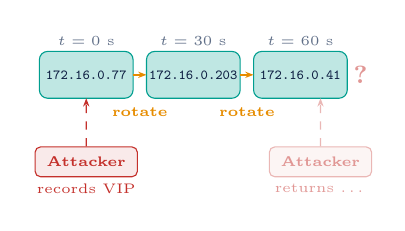
\begin{tikzpicture}[scale=0.85]
        % Three VIP boxes on timeline
        \fill[Teal!25,rounded corners=3pt](0,0.8) rectangle(1.4,1.5);
        \draw[Teal,rounded corners=3pt](0,0.8) rectangle(1.4,1.5);
        \node[font=\tiny\bfseries,text=Navy] at (0.7,1.15){\texttt{172.16.0.77}};
        \fill[Teal!25,rounded corners=3pt](1.6,0.8) rectangle(3.0,1.5);
        \draw[Teal,rounded corners=3pt](1.6,0.8) rectangle(3.0,1.5);
        \node[font=\tiny\bfseries,text=Navy] at (2.3,1.15){\texttt{172.16.0.203}};
        \fill[Teal!25,rounded corners=3pt](3.2,0.8) rectangle(4.6,1.5);
        \draw[Teal,rounded corners=3pt](3.2,0.8) rectangle(4.6,1.5);
        \node[font=\tiny\bfseries,text=Navy] at (3.9,1.15){\texttt{172.16.0.41}};
        % Time labels
        \node[font=\tiny,text=Steel] at(0.7,1.65){$t=0$ s};
        \node[font=\tiny,text=Steel] at(2.3,1.65){$t=30$ s};
        \node[font=\tiny,text=Steel] at(3.9,1.65){$t=60$ s};
        % Rotation arrows
        \draw[Amber,-{Stealth[length=3pt]},line width=0.9pt](1.4,1.15)--(1.6,1.15);
        \draw[Amber,-{Stealth[length=3pt]},line width=0.9pt](3.0,1.15)--(3.2,1.15);
        \node[font=\tiny\bfseries,text=Amber] at(1.5,0.6){rotate};
        \node[font=\tiny\bfseries,text=Amber] at(3.1,0.6){rotate};
        % Attacker scan 1
        \node[draw=Crimson,fill=Crimson!10,rounded corners=2pt,
              font=\tiny\bfseries,text=Crimson,
              minimum width=1.3cm,minimum height=0.38cm](a1) at(0.7,-0.15){Attacker};
        \draw[-{Stealth[length=3pt]},Crimson,dashed](a1.north)--(0.7,0.8);
        \node[font=\tiny,text=Crimson] at(0.7,-0.55){records VIP};
        % Attacker scan 2
        \node[draw=Crimson!35,fill=Crimson!5,rounded corners=2pt,
              font=\tiny\bfseries,text=Crimson!50,
              minimum width=1.3cm,minimum height=0.38cm](a2) at(4.2,-0.15){Attacker};
        \draw[-{Stealth[length=3pt]},Crimson!35,dashed](a2.north)--(4.2,0.8);
        \node[font=\small\bfseries,text=Crimson!50] at(4.8,1.15){\textbf{?}};
        \node[font=\tiny,text=Crimson!50] at(4.2,-0.55){returns \ldots};
      \end{tikzpicture}
    \end{column}
  \end{columns}
\end{frame}

%% ══════════════════════════════════════════════════════════════
%% 02 LITERATURE REVIEW
%% ══════════════════════════════════════════════════════════════
\begin{frame}[shrink=8]{Literature Review}
  \vspace{0.05cm}
  {\scriptsize\renewcommand{\arraystretch}{1.35}\setlength{\tabcolsep}{4pt}
  \begin{tabularx}{\textwidth}{%
      >{\RaggedRight\bfseries}p{3.1cm}
      >{\RaggedRight}p{2.1cm}
      >{\RaggedRight}p{2.3cm}
      >{\RaggedRight\color{Teal!80!black}}p{2.2cm}
      >{\RaggedRight\color{Crimson}}X}
    \rowcolor{Navy}
    \color{white}\bfseries Paper Title &
    \color{white}\bfseries Publisher \& Year &
    \color{white}\bfseries Technology Used &
    \color{white}\bfseries Pros &
    \color{white}\bfseries Gaps / Cons \\[2pt]
    \rowcolor{TealLight!55}
    OF-RHM: Transparent MTD via SDN &
    ACM HotSDN, 2012 &
    OpenFlow 1.0, Ryu SDN &
    First SDN-based IP hopping; hosts unaware &
    No atomic NAT transitions; brief gap window exploitable \\[3pt]
    Towards a Theory of Moving Target Defense &
    ACM CCS Wkshp, 2014 &
    Game theory, formal modelling &
    Strong theoretical foundation for MTD effectiveness &
    No real-time SDN implementation \\[3pt]
    \rowcolor{TealLight!55}
    CHAOS: SDN-Based MTD System &
    Sec.\ Comm.\ Networks, 2017 &
    OpenFlow, NOX controller &
    Reduces scan success rate by over 90\% &
    No barrier synchronisation or physical indicators \\[3pt]
    MTD-Based DDoS Mitigation in SDN &
    IFIP NETWORKING, 2019 &
    SDN, OpenFlow flow tables &
    Combines MTD with active DDoS defence &
    Overhead unmeasured; atomic swap not considered \\[3pt]
    \rowcolor{TealLight!55}
    Evaluation of Network-Level MTD &
    ACM AsiaCCS, 2021 &
    IP randomisation, emulation &
    Quantifies attacker success vs.\ baseline &
    Lab-only; no embedded or Pi platform testing \\
  \end{tabularx}}
\end{frame}

%% ══════════════════════════════════════════════════════════════
%% 03 OBJECTIVES & SIGNIFICANCE
%% ══════════════════════════════════════════════════════════════
\begin{frame}{Objectives of the Project}
  \begin{columns}[T]
    \begin{column}{0.49\textwidth}
      \begin{block}{Primary Objectives}
        \begin{enumerate}\small\setlength\itemsep{5pt}
          \item Build a full OF-RHM controller on \textbf{Raspberry Pi 5} using Ryu SDN and Mininet.
          \item Implement a \textbf{3-table OpenFlow 1.3 pipeline} for transparent IP address translation.
          \item Detect and respond to port-scan attacks in \textbf{under 1 second}.
          \item Provide \textbf{physical LED indicators} for rotation and detection events.
          \item Run an automated demo that \textbf{proves IP addresses change} between two consecutive scans.
        \end{enumerate}
      \end{block}
    \end{column}
    \begin{column}{0.49\textwidth}
      \begin{exampleblock}{Novel Contribution (Next Phase)}
        \begin{itemize}\small\setlength\itemsep{5pt}
          \item Introduce \textbf{NAT Atomicity} --- a two-phase, barrier-synchronised VIP swap that eliminates the transition window present in every prior OF-RHM implementation.
          \item Prove the improvement with \textbf{live iperf3 traffic measurements} during rotation.
          \item First open-source OF-RHM system with a \emph{provably gap-free} rotation.
        \end{itemize}
      \end{exampleblock}
      \vspace{0.2cm}
      \begin{alertblock}{Success Criterion}
        \small\centering Zero IP address overlap between two nmap scans separated by a rotation event.
      \end{alertblock}
    \end{column}
  \end{columns}
\end{frame}

\begin{frame}{Significance of the Project}
  \begin{columns}[T]
    \begin{column}{0.52\textwidth}
      \begin{itemize}\setlength\itemsep{7pt}
        \item \textbf{Proactive, not reactive:} MTD prevents reconnaissance from being useful rather than blocking attacks after they begin.
        \item \textbf{Zero user disruption:} All address translation happens invisibly inside the network switch --- legitimate traffic is never interrupted.
        \item \textbf{Asymmetric cost:} The defender runs a 30-second timer; the attacker must re-scan continuously, multiplying their effort indefinitely.
        \item \textbf{Commodity hardware:} The entire system runs on a \$80 Raspberry Pi 5 with open-source software --- no proprietary appliances needed.
        \item \textbf{Fills a research gap:} Every published OF-RHM system has an unaddressed rotation gap; our next phase is the first to formally eliminate it.
      \end{itemize}
    \end{column}
    \begin{column}{0.44\textwidth}
      \vspace{0.4cm}
      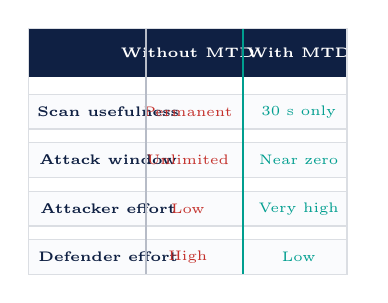
\begin{tikzpicture}[scale=0.88]
        % Simple comparison table
        \fill[Navy] (0,3.5) rectangle(4.6,4.2);
        \node[font=\tiny\bfseries,text=white] at(1.15,3.85){};
        \node[font=\tiny\bfseries,text=white] at(2.3,3.85){Without MTD};
        \node[font=\tiny\bfseries,text=white] at(3.9,3.85){With MTD};
        \foreach \row/\lbl/\bad/\good in {
          3.0/{Scan usefulness}/{Permanent}/{30 s only},
          2.3/{Attack window}/{Unlimited}/{Near zero},
          1.6/{Attacker effort}/{Low}/{Very high},
          0.9/{Defender effort}/{High}/{Low}}{
          \fill[Snow] (0,\row-0.25) rectangle(4.6,\row+0.25);
          \draw[Navy!15] (0,\row-0.25) rectangle(4.6,\row+0.25);
          \node[font=\tiny\bfseries,text=Navy] at(1.15,\row){\lbl};
          \node[font=\tiny,text=Crimson] at(2.3,\row){\bad};
          \node[font=\tiny,text=Teal] at(3.9,\row){\good};
        }
        \draw[Teal,line width=0.6pt] (3.1,0.65) -- (3.1,4.2);
        \draw[Navy!30,line width=0.6pt] (1.7,0.65) -- (1.7,4.2);
        \draw[Navy!15,line width=0.6pt] (0,0.65) rectangle(4.6,4.2);
      \end{tikzpicture}
    \end{column}
  \end{columns}
\end{frame}

%% ══════════════════════════════════════════════════════════════
%% 04 PROBLEM STATEMENT
%% ══════════════════════════════════════════════════════════════
\begin{frame}{Problem Statement}{What Problem Are We Solving?}
  \begin{columns}[T]
    \begin{column}{0.53\textwidth}
      \begin{block}{The Core Problem}
        \begin{itemize}\small\setlength\itemsep{5pt}
          \item Traditional networks assign \textbf{permanent IP addresses} to every device.
          \item Attackers exploit this by scanning once to build a complete network map, then using that map \textbf{at any time in the future}.
          \item The knowledge from a single 5-second scan remains \textbf{valid indefinitely} --- giving the attacker an unlimited window of opportunity.
          \item No existing open-source SDN implementation eliminates the \textbf{brief gap} during rotation when no NAT rules are active.
        \end{itemize}
      \end{block}
    \end{column}
    \begin{column}{0.44\textwidth}
      \vspace{0.2cm}
      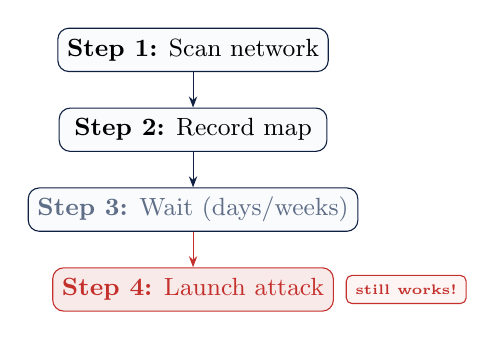
\begin{tikzpicture}[
          ev/.style={draw=Navy,rounded corners=4pt,fill=Snow,
            minimum width=3.4cm,minimum height=0.55cm,
            font=\small,align=center}]
        \node[ev](s1){\textbf{Step 1:} Scan network};
        \node[ev,below=0.45cm of s1](m){\textbf{Step 2:} Record map};
        \node[ev,below=0.45cm of m,text=Steel](w)
          {\textbf{Step 3:} Wait (days/weeks)};
        \node[ev,below=0.45cm of w,draw=Crimson,
              fill=Crimson!10,text=Crimson](a)
          {\textbf{Step 4:} Launch attack};
        \draw[-{Stealth[length=4pt]},Navy] (s1)--(m);
        \draw[-{Stealth[length=4pt]},Navy] (m)--(w);
        \draw[-{Stealth[length=4pt]},Crimson] (w)--(a);
        \node[draw=Crimson,rounded corners=2pt,font=\tiny\bfseries,
              text=Crimson,fill=Crimson!5,right=0.15cm of a]
          {still works!};
      \end{tikzpicture}
    \end{column}
  \end{columns}
\end{frame}

\begin{frame}{Problem Statement}{Why Is This Important?}
  \begin{columns}[T]
    \begin{column}{0.54\textwidth}
      \begin{itemize}\setlength\itemsep{6pt}
        \item \textbf{Reconnaissance-based attacks} account for a large share of successful network breaches --- identifying live hosts and open ports is always the first step.
        \item \textbf{IoT and edge devices} (like Raspberry Pi) are deployed in sensitive settings but receive the weakest security coverage.
        \item \textbf{Firewalls and IDS} cannot prevent an attacker from passively mapping the network --- they only block or alert on active attacks.
        \item \textbf{The transition gap} in existing OF-RHM implementations is an unaddressed vulnerability: during rotation, real IP addresses may be briefly exposed.
      \end{itemize}
    \end{column}
    \begin{column}{0.42\textwidth}
      \begin{exampleblock}{Real-World Example}
        \small If a hospital deployed medical devices on a static-IP network, an attacker could map the network once and return during a critical moment. MTD forces continuous re-scanning --- dramatically raising effort and detection risk.
      \end{exampleblock}
      \vspace{0.25cm}
      \begin{alertblock}{The Transition Gap}
        \small During each rotation, there is a window of \textbf{50--200\,ms} where the switch has no NAT rules. Any packet that arrives in this window is misrouted or exposes real IP addresses.
      \end{alertblock}
    \end{column}
  \end{columns}
\end{frame}

%% ══════════════════════════════════════════════════════════════
%% 05 KEY DELIVERABLES
%% ══════════════════════════════════════════════════════════════
\begin{frame}{Key Deliverables \& Milestones}
  \begin{columns}[T]
    \begin{column}{0.56\textwidth}
      {\small\renewcommand{\arraystretch}{1.4}\setlength{\tabcolsep}{5pt}
      \begin{tabularx}{\linewidth}{>{\bfseries\color{Navy}\centering}p{0.5cm}
          >{\RaggedRight}X >{\centering\arraybackslash}p{1.8cm}}
        \rowcolor{Navy}
        \color{white}\# &
        \color{white}Deliverable &
        \color{white}Status \\
        \rowcolor{TealLight!55}
        D1 & Ryu controller with 3-table OpenFlow 1.3 pipeline &
          {\color{Teal}\bfseries\small Done} \\
        D2 & VIP assignment \& automatic host learning &
          {\color{Teal}\bfseries\small Done} \\
        \rowcolor{TealLight!55}
        D3 & 30-second scheduled VIP rotation &
          {\color{Teal}\bfseries\small Done} \\
        D4 & Real-time scan detection \& emergency rotation &
          {\color{Teal}\bfseries\small Done} \\
        \rowcolor{TealLight!55}
        D5 & GPIO LED indicators (green + blue) &
          {\color{Teal}\bfseries\small Done} \\
        D6 & Automated demo with PASS/FAIL verification &
          {\color{Teal}\bfseries\small Done} \\
        \rowcolor{TealLight!55}
        D7 & NAT-atomic two-phase rotation (novelty) &
          {\color{Amber}\bfseries\small Next phase} \\
      \end{tabularx}}
    \end{column}
    \begin{column}{0.4\textwidth}
      \vspace{0.5cm}\centering
      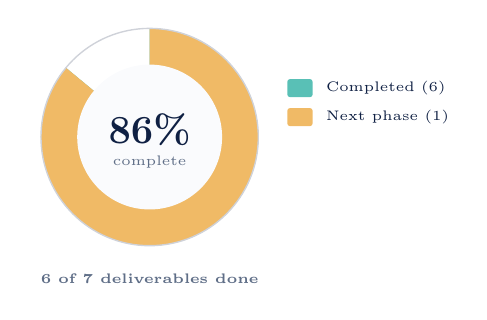
\begin{tikzpicture}[scale=0.92]
        % Donut chart — 86% done
        \fill[Teal!65] (0,0) -- (90:1.5cm) arc(90:-219.6:1.5cm) -- cycle;
        \fill[Amber!60] (0,0) -- (-219.6:1.5cm) arc(-219.6:90:1.5cm) -- cycle;
        \fill[Snow] (0,0) circle(1.0cm);
        \draw[Navy!20,line width=0.5pt] (0,0) circle(1.5cm);
        \node[font=\Large\bfseries,text=Navy] at(0,0.1){86\%};
        \node[font=\tiny,text=Steel] at(0,-0.35){complete};
        % legend
        \fill[Teal!65,rounded corners=1pt](1.9,0.55) rectangle(2.25,0.8);
        \node[font=\tiny,text=Navy,right] at(2.3,0.67){Completed (6)};
        \fill[Amber!60,rounded corners=1pt](1.9,0.15) rectangle(2.25,0.4);
        \node[font=\tiny,text=Navy,right] at(2.3,0.27){Next phase (1)};
        \node[font=\tiny\bfseries,text=Steel] at(0,-1.95){6 of 7 deliverables done};
      \end{tikzpicture}
    \end{column}
  \end{columns}
\end{frame}

%% ══════════════════════════════════════════════════════════════
%% 06 METHODOLOGY
%% ══════════════════════════════════════════════════════════════
\begin{frame}{Methodology}{System Architecture}
  \begin{columns}[T]
    \begin{column}{0.46\textwidth}
      \begin{itemize}\small\setlength\itemsep{5pt}
        \item All components run on a single \textbf{Raspberry Pi 5}.
        \item \textbf{Mininet} creates a virtual network: 3 hosts + 1 attacker + 1 switch, using real Linux networking.
        \item \textbf{Ryu SDN Controller} programs the switch in real time via OpenFlow 1.3 messages.
        \item \textbf{Open vSwitch (OVS)} executes flow rules; packets with no matching rule are forwarded to the controller.
        \item \textbf{LED indicators} on GPIO pins give live physical feedback during demos.
      \end{itemize}
    \end{column}
    \begin{column}{0.52\textwidth}
      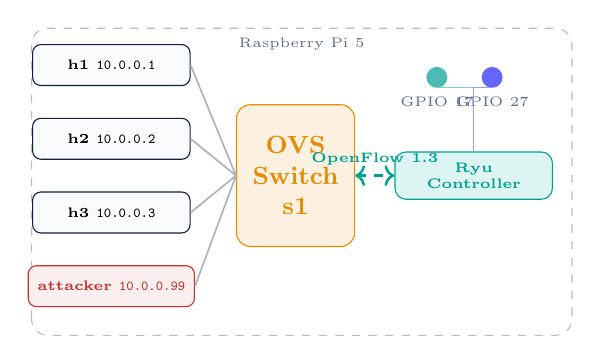
\begin{tikzpicture}[scale=0.78,
          host/.style={draw=Navy,fill=Snow,rounded corners=3pt,
            minimum width=2.0cm,minimum height=0.52cm,
            font=\tiny\bfseries,align=center},
          sw/.style={draw=Amber,fill=Amber!12,rounded corners=5pt,
            minimum width=1.5cm,minimum height=1.8cm,
            font=\small\bfseries,text=Amber,align=center},
          ctrl/.style={draw=Teal,fill=TealLight,rounded corners=4pt,
            minimum width=2.0cm,minimum height=0.6cm,
            font=\tiny\bfseries,text=Teal,align=center}]
        % Pi border
        \draw[Navy!30,dashed,rounded corners=6pt]
          (-0.3,-0.4) rectangle(8.5,4.6);
        \node[font=\tiny,text=Steel] at(4.1,4.35){Raspberry Pi 5};
        % Hosts
        \node[host](h1) at(1.0,4.0){h1 \texttt{10.0.0.1}};
        \node[host](h2) at(1.0,2.8){h2 \texttt{10.0.0.2}};
        \node[host](h3) at(1.0,1.6){h3 \texttt{10.0.0.3}};
        \node[host,draw=Crimson,text=Crimson,fill=Crimson!8]
          (atk) at(1.0,0.4){attacker \texttt{10.0.0.99}};
        % Switch
        \node[sw](sw) at(4.0,2.2){OVS\\Switch\\s1};
        % Controller
        \node[ctrl](ctrl) at(6.9,2.2){Ryu\\Controller};
        % LED dots
        \fill[Teal!70] (6.3,3.8) circle(0.17cm);
        \fill[blue!60]  (7.2,3.8) circle(0.17cm);
        \node[font=\tiny,text=Steel] at(6.3,3.4){GPIO 17};
        \node[font=\tiny,text=Steel] at(7.2,3.4){GPIO 27};
        % Lines
        \foreach \n in {h1,h2,h3,atk}
          \draw[Navy!35,line width=0.6pt] (\n.east) -- (sw.west);
        \draw[Teal,<->,dashed,line width=0.9pt]
          (sw.east) -- (ctrl.west)
          node[midway,above,font=\tiny\bfseries,text=Teal]
          {OpenFlow 1.3};
        \draw[Teal!50,thin] (ctrl.north) |- (6.3,3.63);
        \draw[blue!40,thin] (ctrl.north) |- (7.2,3.63);
      \end{tikzpicture}
    \end{column}
  \end{columns}
\end{frame}

\begin{frame}{Methodology}{The 3-Table OpenFlow Pipeline}
  \vspace{0.1cm}
  \centering
  \begin{tikzpicture}[scale=0.85,
      tbl/.style={draw=Navy,fill=Navy!7,rounded corners=6pt,
        minimum width=3.0cm,minimum height=2.3cm,align=center,
        font=\small},
      pkt/.style={draw,rounded corners=3pt,minimum width=1.8cm,
        minimum height=0.5cm,font=\small\bfseries,align=center}]
    \node[pkt,draw=Amber,fill=Amber!12](in) at(-2.3,0)
      {Packet\\arrives};
    \node[tbl](t0) at(1.1,0){
      \textcolor{Navy}{\bfseries\small Table 0}\\[3pt]
      \textcolor{Teal}{\small Outbound NAT}\\[6pt]
      \textcolor{Steel}{\footnotesize Hide real\\source IP\\with VIP}
    };
    \node[tbl](t1) at(4.9,0){
      \textcolor{Navy}{\bfseries\small Table 1}\\[3pt]
      \textcolor{Teal}{\small Inbound NAT}\\[6pt]
      \textcolor{Steel}{\footnotesize Translate\\VIP dst\\to real IP}
    };
    \node[tbl](t2) at(8.7,0){
      \textcolor{Navy}{\bfseries\small Table 2}\\[3pt]
      \textcolor{Teal}{\small L2 Forward}\\[6pt]
      \textcolor{Steel}{\footnotesize Deliver by\\MAC address}
    };
    \node[pkt,draw=Teal,fill=TealLight,text=Teal](out) at(11.8,0)
      {Packet\\delivered};
    \draw[-{Stealth[length=5pt]},Navy,line width=1.2pt](in)--(t0);
    \draw[-{Stealth[length=5pt]},Navy,line width=1.2pt](t0)--(t1);
    \draw[-{Stealth[length=5pt]},Navy,line width=1.2pt](t1)--(t2);
    \draw[-{Stealth[length=5pt]},Teal,line width=1.2pt](t2)--(out);
    % annotations below
    \node[font=\tiny,align=center,text=Navy] at(1.1,-1.7)
      {\texttt{src: 10.0.0.1}\\$\downarrow$\\\textcolor{Teal}{\texttt{src: 172.16.0.77}}};
    \node[font=\tiny,align=center,text=Navy] at(4.9,-1.7)
      {\texttt{dst: 172.16.0.77}\\$\downarrow$\\\textcolor{Teal}{\texttt{dst: 10.0.0.2}}};
    \node[font=\tiny,align=center,text=Navy] at(8.7,-1.7)
      {out-port: 2};
    % TCP copy
    \draw[-{Stealth[length=3pt]},Crimson,dashed,line width=0.7pt]
      (t1.north) -- ++(0,0.8)
      node[above,font=\tiny\bfseries,text=Crimson,align=center]
        {TCP SYN copy\\$\rightarrow$ controller};
  \end{tikzpicture}
  \vspace{0.3cm}
  {\footnotesize\color{Steel}
    Each packet passes through all three tables in order. The controller only intervenes when no rule matches.}
\end{frame}

\begin{frame}{Methodology}{Tools, Techniques \& Parameters}
  \begin{columns}[T]
    \begin{column}{0.49\textwidth}
      \begin{block}{Software Stack}
        \begin{itemize}\small\setlength\itemsep{4pt}
          \item \textbf{Python 3 + Ryu:} SDN controller framework; all OpenFlow message handling.
          \item \textbf{Mininet:} Network emulator; virtual hosts with real Linux networking.
          \item \textbf{Open vSwitch:} Virtual switch inside Mininet executing flow rules.
          \item \textbf{lgpio:} GPIO library for Pi 5; controls LED indicators.
          \item \textbf{nmap:} Port-scan tool used by the attacker script to probe VIPs.
          \item \textbf{eventlet:} Async library used by Ryu; requires subprocess isolation for GPIO.
        \end{itemize}
      \end{block}
    \end{column}
    \begin{column}{0.49\textwidth}
      \begin{exampleblock}{Key Configuration}
        \begin{itemize}\small\setlength\itemsep{4pt}
          \item \textbf{VIP Pool:} 172.16.0.0/24 — 254 available fake addresses
          \item \textbf{Rotation interval:} 30 seconds (scheduled), or immediate on scan
          \item \textbf{Scan threshold:} 1 TCP SYN to any VIP triggers detection
          \item \textbf{Scan window:} 10-second sliding window
          \item \textbf{NAT rule priority:} 10 (new rules at 110 during atomic swap)
          \item \textbf{Controller port:} 6653
        \end{itemize}
      \end{exampleblock}
    \end{column}
  \end{columns}
\end{frame}

%% ══════════════════════════════════════════════════════════════
%% 07 PROGRESS
%% ══════════════════════════════════════════════════════════════
\begin{frame}{Progress So Far}{What Has Been Built}
  \begin{columns}[T]
    \begin{column}{0.54\textwidth}
      \begin{itemize}\setlength\itemsep{6pt}
        \item[$\checkmark$] \textbf{Full controller:} 3-table pipeline, ARP proxy, VIP assignment and scheduled rotation all working on Pi 5.
        \item[$\checkmark$] \textbf{Scan detection:} Emergency rotation fires within \textbf{1 second} of the first TCP SYN to any VIP.
        \item[$\checkmark$] \textbf{LED system:} Green blinks once per rotation; blue blinks 3$\times$ per scan alert. Timing isolated via child subprocess to bypass eventlet interference.
        \item[$\checkmark$] \textbf{Automated demo:} Builds network, runs two nmap scans 35 seconds apart, compares results, and prints PASS or FAIL.
        \item[$\checkmark$] \textbf{Consistent result:} Demo produces \emph{zero IP overlap} between scans every run.
      \end{itemize}
    \end{column}
    \begin{column}{0.42\textwidth}
      \vspace{0.35cm}
      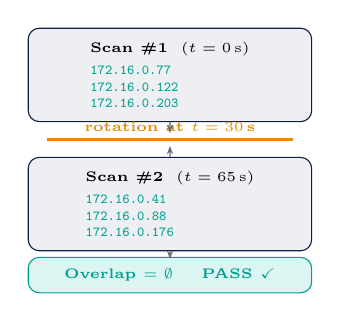
\begin{tikzpicture}[scale=0.82,
          res/.style={draw=Navy,fill=Navy!7,rounded corners=4pt,
            minimum width=3.6cm,font=\tiny,inner sep=5pt,align=left}]
        \node[res](s1) at(1.8,3.5){
          \textbf{Scan \#1} \ ($t=0$\,s)\\[2pt]
          \textcolor{Teal}{\texttt{172.16.0.77}}\\
          \textcolor{Teal}{\texttt{172.16.0.122}}\\
          \textcolor{Teal}{\texttt{172.16.0.203}}
        };
        \node[res](s2) at(1.8,1.5){
          \textbf{Scan \#2} \ ($t=65$\,s)\\[2pt]
          \textcolor{Teal}{\texttt{172.16.0.41}}\\
          \textcolor{Teal}{\texttt{172.16.0.88}}\\
          \textcolor{Teal}{\texttt{172.16.0.176}}
        };
        \draw[Amber,line width=1.2pt](-0.1,2.5)--(3.7,2.5);
        \node[font=\tiny\bfseries,text=Amber] at(1.8,2.7){rotation at $t=30$\,s};
        \draw[Steel,dashed,-{Stealth[length=3pt]}](s1.south)--(1.8,2.6);
        \draw[Steel,dashed,-{Stealth[length=3pt]}](s2.north)--(1.8,2.4);
        \node[draw=Teal,fill=TealLight,rounded corners=4pt,
              minimum width=3.6cm,minimum height=0.45cm,
              font=\tiny\bfseries,text=Teal] at(1.8,0.4)
          {Overlap $=\emptyset$ \quad \textbf{PASS $\checkmark$}};
        \draw[Steel,dashed,-{Stealth[length=3pt]}](s2.south)--(1.8,0.65);
      \end{tikzpicture}
    \end{column}
  \end{columns}
\end{frame}

\begin{frame}{Progress So Far}{Solving the LED Timing Challenge}
  \begin{columns}[T]
    \begin{column}{0.48\textwidth}
      \begin{alertblock}{Problem: Eventlet Interference}
        \small Ryu uses \textbf{eventlet} which replaces Python's \texttt{time.sleep()} with a cooperative version. This caused LED blink loops to complete in microseconds --- producing a single flicker instead of three distinct blinks. Multiple rapid scan packets also spawned concurrent processes that conflicted over the same GPIO pin.
      \end{alertblock}
      \vspace{0.2cm}
      \begin{exampleblock}{Solution: Subprocess Isolation}
        \small Each blink sequence runs in a \textbf{separate child process} launched with \texttt{subprocess.Popen()}. The child has standard Python timing. A \textbf{2-second cooldown} prevents concurrent processes from conflicting.
      \end{exampleblock}
    \end{column}
    \begin{column}{0.48\textwidth}
      \vspace{0.3cm}
      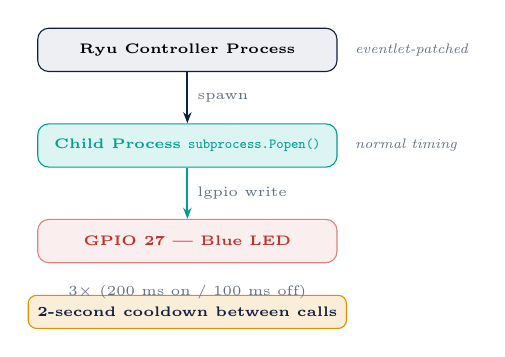
\begin{tikzpicture}[scale=0.82,
          box/.style={draw=Navy,fill=Navy!7,rounded corners=4pt,
            minimum width=3.8cm,minimum height=0.55cm,
            font=\tiny\bfseries,align=center}]
        \node[box](ctrl){Ryu Controller Process};
        \node[font=\tiny,text=Steel,right=0.1cm of ctrl]
          {\itshape eventlet-patched};
        \node[box,below=0.65cm of ctrl,draw=Teal,
              fill=TealLight,text=Teal](child)
          {Child Process \texttt{subprocess.Popen()}};
        \node[font=\tiny,text=Steel,right=0.1cm of child]
          {\itshape normal timing};
        \node[box,below=0.65cm of child,draw=Crimson!60,
              fill=Crimson!8,text=Crimson](gpio)
          {GPIO 27 — Blue LED};
        \draw[-{Stealth[length=4pt]},Navy,line width=0.8pt]
          (ctrl)--(child)
          node[midway,right,font=\tiny,text=Steel]{spawn};
        \draw[-{Stealth[length=4pt]},Teal,line width=0.8pt]
          (child)--(gpio)
          node[midway,right,font=\tiny,text=Steel]{lgpio write};
        \node[draw=Amber,fill=Amber!15,rounded corners=3pt,
              font=\tiny\bfseries,text=Navy,
              minimum width=3.8cm,minimum height=0.42cm,
              below=0.4cm of gpio]
          {2-second cooldown between calls};
        \node[font=\tiny,text=Steel,below=0.15cm of gpio]
          {3$\times$ (200 ms on / 100 ms off)};
      \end{tikzpicture}
    \end{column}
  \end{columns}
\end{frame}

%% ══════════════════════════════════════════════════════════════
%% 08 CHALLENGES
%% ══════════════════════════════════════════════════════════════
\begin{frame}{Challenges \& Risks}
  \begin{columns}[T]
    \begin{column}{0.5\textwidth}
      \begin{block}{Challenges Encountered}
        \begin{itemize}\small\setlength\itemsep{5pt}
          \item \textbf{Eventlet timing:} Ryu's async library disrupted GPIO timing; required subprocess isolation to fix.
          \item \textbf{Concurrent subprocess conflicts:} Multiple rapid scans triggered multiple blink processes competing over the same GPIO pin; fixed with cooldown.
          \item \textbf{REST API hang:} Adding Ryu's built-in REST server caused a silent controller deadlock --- removed entirely.
          \item \textbf{VIP pool size:} A /16 pool (65,534 addresses) made nmap scans unreliable in demo time; reduced to /24 (254 addresses).
        \end{itemize}
      \end{block}
    \end{column}
    \begin{column}{0.46\textwidth}
      \begin{alertblock}{Risks Going Forward}
        \begin{itemize}\small\setlength\itemsep{5pt}
          \item \textbf{Transition gap:} Current rotation briefly exposes real IPs between rule deletion and installation --- the primary target for next phase.
          \item \textbf{Barrier timing:} The atomic swap requires the switch to reply to a barrier request promptly; not guaranteed under high traffic load.
          \item \textbf{Platform lock-in:} The lgpio library is Pi 5 specific and not portable to other platforms.
          \item \textbf{Scale:} Demo uses 4 hosts --- behaviour with 100+ hosts and many simultaneous scans is untested.
        \end{itemize}
      \end{alertblock}
    \end{column}
  \end{columns}
\end{frame}

%% ══════════════════════════════════════════════════════════════
%% 09 NEXT STEPS
%% ══════════════════════════════════════════════════════════════
\begin{frame}{Next Steps}
  \begin{columns}[T]
    \begin{column}{0.52\textwidth}
      \begin{block}{Short-Term Tasks}
        \begin{enumerate}\small\setlength\itemsep{5pt}
          \item \textbf{Implement NAT atomicity:} Install new VIP rules at priority 110, wait for \texttt{OFPT\_BARRIER\_REPLY}, then delete old rules at priority 10. Zero-gap rotation.
          \item \textbf{Measure the gap:} Run iperf3 during rotation to count dropped or misrouted packets before and after the fix.
          \item \textbf{Document the contribution:} Compare measured results against all published OF-RHM papers to confirm this is the first gap-free implementation.
          \item \textbf{Robustness tests:} Verify correct behaviour with 10+ simultaneous scanners and under heavy background traffic.
        \end{enumerate}
      \end{block}
    \end{column}
    \begin{column}{0.45\textwidth}
      \vspace{0.25cm}
      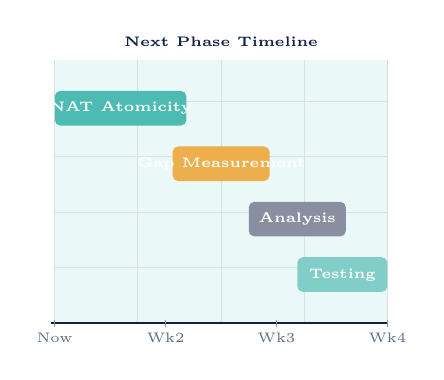
\begin{tikzpicture}[scale=0.88]
        % Gantt chart
        \fill[TealLight!60] (0,0) rectangle(4.8,3.8);
        \draw[Navy!15,line width=0.4pt] (0,0) grid[ystep=0.8,xstep=1.2](4.8,3.8);
        % Bars
        \fill[Teal!70,rounded corners=2pt] (0.0,2.85) rectangle(1.9,3.35);
        \fill[Amber!70,rounded corners=2pt] (1.7,2.05) rectangle(3.1,2.55);
        \fill[Navy!50,rounded corners=2pt] (2.8,1.25) rectangle(4.2,1.75);
        \fill[Teal!50,rounded corners=2pt] (3.5,0.45) rectangle(4.8,0.95);
        % Bar labels
        \node[font=\tiny\bfseries,text=white] at(0.95,3.10){NAT Atomicity};
        \node[font=\tiny\bfseries,text=white] at(2.40,2.30){Gap Measurement};
        \node[font=\tiny\bfseries,text=white] at(3.50,1.50){Analysis};
        \node[font=\tiny\bfseries,text=white] at(4.15,0.70){Testing};
        % Time axis
        \draw[Navy,line width=0.8pt](-0.05,0) -- (4.8,0);
        \foreach \x/\lbl in {0/Now, 1.6/Wk2, 3.2/Wk3, 4.8/Wk4}{
          \draw[Navy!50,line width=0.5pt](\x,-0.05)--(\x,0.05);
          \node[font=\tiny,text=Steel,below]at(\x,0){\lbl};
        }
        \node[font=\tiny\bfseries,text=Navy,above] at(2.4,3.85)
          {Next Phase Timeline};
      \end{tikzpicture}
    \end{column}
  \end{columns}
\end{frame}

%% ══════════════════════════════════════════════════════════════
%% 10 CONCLUSION
%% ══════════════════════════════════════════════════════════════
\begin{frame}{Conclusion \& Summary}
  \begin{columns}[T]
    \begin{column}{0.54\textwidth}
      \begin{itemize}\setlength\itemsep{6pt}
        \item A \textbf{fully functional Moving Target Defense system} has been built and demonstrated on Raspberry Pi 5.
        \item The system detects port scans within \textbf{1 second} and immediately rotates all virtual IPs, rendering reconnaissance useless.
        \item The automated demo \textbf{consistently passes} --- zero address overlap between consecutive scans.
        \item \textbf{NAT atomicity} (next phase) will be the first provably gap-free VIP rotation in any open-source OF-RHM implementation.
        \item This project shows that \textbf{proactive, dynamic security} is achievable on commodity hardware at minimal cost.
      \end{itemize}
    \end{column}
    \begin{column}{0.43\textwidth}
      \vspace{0.2cm}
      \begin{exampleblock}{Key Takeaways}
        \begin{itemize}\small\setlength\itemsep{4pt}
          \item Attackers depend on \emph{static} information --- remove that and their advantage collapses.
          \item SDN makes dynamic, programmable security practical on real hardware today.
          \item Atomicity turns a good system into a \textbf{provably correct} one.
        \end{itemize}
      \end{exampleblock}
      \vspace{0.35cm}
      \centering
      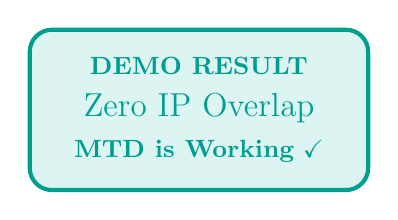
\begin{tikzpicture}
        \node[draw=Teal,fill=TealLight,rounded corners=8pt,
              line width=1.5pt,inner xsep=16pt,inner ysep=10pt,
              font=\small,align=center,text=Teal]{
          \textbf{DEMO RESULT}\\[4pt]
          {\large Zero IP Overlap}\\[4pt]
          \textbf{MTD is Working} $\checkmark$
        };
      \end{tikzpicture}
    \end{column}
  \end{columns}
\end{frame}

%% ── Q & A ────────────────────────────────────────────────────
{\darkbg
\setbeamertemplate{footline}{}
\begin{frame}[plain]
  \vspace{1.8cm}
  \centering
  {\color{Teal}\fontsize{36}{40}\selectfont\bfseries Questions?}\\[0.5cm]
  {\color{white}\large\itshape We welcome your feedback and discussion.}\\[1.4cm]
  {\color{TealLight}\small
    \renewcommand{\arraystretch}{1.5}
    \begin{tabular}{rl}
      \bfseries Project: &
        Moving Target Defense via OF-RHM \\
      \bfseries Platform: &
        Raspberry Pi 5 \textbullet\ Ryu \textbullet\ Mininet \textbullet\ OpenFlow 1.3 \\
      \bfseries Contact: &
        Aditi Sriram --- oopsitsjustus@gmail.com \\
    \end{tabular}
  }\\[1.6cm]
  {\color{white}\Large\bfseries Thank You}\\[0.15cm]
  {\color{TealLight}\small for your attention}
\end{frame}}

%% ── REFERENCES ───────────────────────────────────────────────
\begin{frame}[allowframebreaks]{References}
  \vspace{0.1cm}
  {\footnotesize\setlength\itemsep{6pt}
  \begin{enumerate}
    \item J.\,H. Jafarian, E. Al-Shaer, and Q. Duan,
      ``OpenFlow Random Host Mutation: Transparently Moving Target Defense
      using Software Defined Networking,''
      \textit{Proc.\ ACM SIGCOMM Workshop on HotSDN}, 2012.

    \item S. Jajodia, A.\,K. Ghosh, V. Swarup, C. Wang, and X.\,S. Wang (Eds.),
      \textit{Moving Target Defense: Creating Asymmetric Uncertainty for Cyber Threats.}
      Springer, 2011.

    \item L. Shi, X. Li, T. Yu, J. Lu, and H. Lu,
      ``CHAOS: An SDN-Based Moving Target Defense System,''
      \textit{Security and Communication Networks}, 2017.

    \item M.\,A. Razzaq, M. Hussain, and A.\,H. Pasha,
      ``Software Defined Networking Based MTD for DDoS Mitigation,''
      \textit{Proc.\ IFIP NETWORKING}, 2019.

    \item Y. Han, W. Lu, and S. Bhattacharya,
      ``Analysis and Evaluation of Network-Based Moving Target Defenses,''
      \textit{Proc.\ ACM AsiaCCS}, 2021.
  \end{enumerate}
  \vspace{0.25cm}
  {\color{Steel}
  \textbf{Open-source tools used:}\
    Ryu SDN Framework (osrg/ryu) \textbullet\
    Mininet (mininet/mininet) \textbullet\
    Open vSwitch \textbullet\
    Python 3 \textbullet\
    lgpio \textbullet\
    nmap}}
\end{frame}

\end{document}
